

\section{Implementation}
\label{sec:implementation}

%\begin{wraptable}[11]{r}{0.32\textwidth}
%	\vspace{-1.5em} 
%	\centering
%	\begin{tabular}{@{} l S[table-format=5.0] @{}}
%		\toprule
%		\textbf{Module}                & {\textbf{LoC}} \\
%		\midrule
%		Input \& Parsing               &  1723          \\
%		Model Construction             &  5561          \\
%		Petri--Net Conversion           &   843          \\
%		Reachability          &  2628          \\
%		Proof Checking                 &  3240          \\
%		Utilities                      &  2160          \\
%		Testing \& Evaluation          &  2118          \\
%		\midrule
%		\textbf{Total}                 & \textbf{18273} \\
%		\bottomrule
%	\end{tabular}
%	\caption{Lines of Code}
%	\label{tab:loc_summary2}
%\end{wraptable}
%\vspace{-1.5\baselineskip} % nudge following text up a bit
%We implemented our approach in \toolname{}~\cite{ArtifactRepository}, a publicly available toolchain 
%%consisting of over $18{,}200$ LoC 
%written mostly in \texttt{Rust}. 
%(see Table~\ref{tab:loc_summary2})
%
%
%We next elaborate on the architecture of our tool and the various optimizations we added to allow it to run efficiently.
%For the underlying Petri Net model checker, we use SMPT~\cite{AmDa23},though other off-the-shelf solvers can be used as well.
%For the underlying Petri Net model checker, we use SMPT~\cite{AmDa23} which supports \textit{unbounded} reachability queries (see Appendix~\ref{appendix:smpt}).
%, and which uses Z3 as an underlying SMT solver~\cite{DeBj08}. 
%and which we extended to support our setting (for example, we needed to extend the solver to support proof generation). 
%
%We note that other off-the-shelf solvers can be used as well.

%The implementation..

%\begin{enumerate}
%	\item The extra things we did to make the thing actually run
%	\item Code architecture
%	\item Optimizations
%\end{enumerate}

%\newpage
\subsection{Code Architecture}

%\begin{tabular}{|l|r|}
%	\hline
%	\textbf{Module} & \textbf{LoC} \\
%	\hline
%	Input \& Parsing                             & 1723  \\
%	\hline
%	Model Construction                           & 5561  \\
%	\hline
%	Petri-Net Conversion                         & 843   \\
%	\hline
%	Reachability Checking                        & 2628  \\
%	\hline
%	Proof Checking                               & 3240  \\
%	\hline
%	Utilities                                       & 2160  \\
%	\hline
%	Testing \& Evaluation               & 2118  \\
%	\hline
%	\textbf{Total}                               & \textbf{18273} \\
%	\hline
%\end{tabular}


%
%\begin{table}[ht]
%	\centering
%	\label{tab:loc_summary}
%	\begin{tabular}{@{} l S[table-format=5.0] @{}}
%		\toprule
%		\textbf{Module}                & {\textbf{LoC}} \\
%		\midrule
%		Input \& Parsing               &  1723          \\
%		Model Construction             &  5561          \\
%		Petri–Net Conversion           &   843          \\
%		Reachability Checking          &  2628          \\
%		Proof Checking                 &  3240          \\
%		Utilities                      &  2160          \\
%		Testing \& Evaluation          &  2118          \\
%		\midrule
%		\textbf{Total}                 & \textbf{18273}          \\
%		\bottomrule
%	\end{tabular}
%	\caption{Lines of Code by Module}
%\end{table}
%

% Then, where you want the table wrapped to the right:
%
% this table summarizes the values without whitespaces/comments and without the code for SMPT (or the wrapper) or the carfo and toml files
%
%\begin{wraptable}[8]{r}{0.32\textwidth}
%	\centering
%	\begin{tabular}{@{} l S[table-format=5.0] @{}}
%		\toprule
%		\textbf{Module}                & {\textbf{LoC}} \\
%		\midrule
%		Input \& Parsing               &  1723          \\
%		Model Construction             &  5561          \\
%		Petri–Net Conversion           &   843          \\
%		Reachability          &  2628          \\
%		Proof Checking                 &  3240          \\
%		Utilities                      &  2160          \\
%		Testing \& Evaluation          &  2118          \\
%		\midrule
%		\textbf{Total}                 & \textbf{18273} \\
%		\bottomrule
%	\end{tabular}
%	\caption{Lines of Code (LoC)}
%	\label{tab:loc_summary2}
%\end{wraptable}
%
%\noindent

Our decision procedure is implemented in \toolname{}~\cite{ArtifactRepository}, a publicly available toolchain 
%consisting of over $18{,}200$ LoC 
written mostly in \texttt{Rust}. 
%
The toolchain receives an input program (which can be written in the \toolname{} syntax), and runs the end-to-end serializability checker on it. If the program is serializable, the toolchain returns a network-system level proof thereof; otherwise, if it is not serializable, the toolchain provides a counterexample, i.e., a specific interleaving that induces a multiset of request/response pairs that cannot be obtained in \textit{any} serial execution.
%
Our toolchain reduces the problem of deciding the networks system's serializability to an equivalent Petri net reachability problem over an unbounded number of tokens. Our construction guarantees that (i) the Petri net represents every possible request/response multiset that is induced by an interleaving of the original program; and (ii) the reachability query encodes multisets of request/response pairs that \textit{cannot} be induced by serial executions.
%
In order to cope with the \texttt{Ackermann}-completeness of unbounded Petri net reachability~\cite{CzWo22,Le22}, we implemented the various optimizations that expedite the search procedure, both at the Petri net level, and also, at the property-encoding level.
%
We illustrate the pipeline of \toolname{} in Fig.~\ref{fig:full_program_flow}. Furthermore, \toolname{} includes the following modules:
 

\begin{enumerate}
	\item \textbf{Input \& parsing.} 
	Our toolchain receives as input either a \toolname{} program with the syntax described in~\Cref{sec:problem-definition}, or alternatively, a \texttt{JSON} file that directly encodes a network system. In the case of the former, the toolchain does an additional step in which it parses the input %(using the \texttt{parser.rs} module) 
	to an expression tree that is then translated into the equivalent network system.
%	, represented as a struct in the \texttt{ns.rs} module. 
	
	\item \textbf{Petri net conversion.} The network system is subsequently translated into a Petri net 
%	(see the \texttt{petri.rs} module) 
representing all possible interleavings of the original program as depicted, for example, in Fig.~\ref{fig:code2ExamplePN}.
	Each place represents a state (either global or local) or a response. Each token that is not in a place encoding a global state, represents a single in-flight request or a terminated response. 
Furthermore, we note that the Petri net is encoded in the de facto standard \texttt{NET} format, to allow support by off-the-shelf Petri net model checkers. 
	
	\item \textbf{Semilinear conversion.} 
%	This includes a set of modules (\texttt{kleene.rs}, \texttt{semilinear.rs}, and \texttt{presburger.rs}) which 
We construct a semilinear set that encodes all the request/response multisets that cannot be induced by any serial exection.
This step is done via translation of the serialized NFA (e.g., Fig.~\ref{fig:code2ExampleNFA}) to a regular expression, which is then projected (using the Parikh image) and complemented. 
%	This conversion is done by the following pipeline: (1) the NS is translated to an NFA encoding all possible request/response pairs of the input program; (2) This NFA is translated to a regex (via Kleene's Theorem) and then projected (via the Parikh Image) to a semilinear set. The (finite) encoding of the semilinear set symbolically represents all outputs attained via serializable executions of the program, running for an unbounded number of steps; (3) finally, we complement the semilinear set to encode all outputs unattainable via serial executions. 
	After this stage, our toolchain generates an \texttt{XML}-formatted file encoding a reachability query over the token distribution of the Petri net.
	
	
	\item \textbf{Reachability engine.} Both the Peri net and the accompanying reachability query are fed to a Petri net model checker, which combines techniques such as \textit{bounded model checking} (BMC)~\cite{BiCiClZh99} in search of a counterexample; and \textit{state equation reasoning}~\cite{Mu77} in order to prove non-reachability. 
%	This engine is implemented in the \texttt{reachability.rs} and \texttt{reachability\_with\_proofs.rs}  modules.
	%
	Furthermore, in order to curtail the search space, we replace ``large'' (Petri net, reachability query) pairs with multiple sliced Petri nets, with each sliced Petri net coupled with a sub-query encoding a separate disjunct in the original, full query. 
%	of the original query.
	We iteratively solve the 
	disjuncts on the fly, until either \texttt{SAT} is reached, in which case, we have a concrete counterexample; or otherwise, if all disjuncts are found to be \texttt{UNSAT}, we deduce that the original program is serializable.
	
	
	\item \textbf{Proof \& certification.} 
	If the query is \texttt{SAT}, we reconstruct the reachable marking and validate a network-system level counterexample. Otherwise, if the query is \texttt{UNSAT}, we extract an inductive, per-disjunct proof for non-satisfiability, and then ``stitch'' these to a single inductive serializability certificate. This certificate is then projected to the network system, over which we validate (i) initiation, (ii) inductiveness, and (iii) query refutation.
	%
%	If the query is \texttt{SAT}, we reconstruct a non-serializable NS-level execution and validate its correctness. Otherwise, if all disjuncts are \texttt{UNSAT}, our proof module extracts a separate proof for each disjunct. We subsequently ``stitch'' these proofs to a single inductive invariant, and project it to the NS-level, representing a full inductive proof certificate for serializability. Our checker also validates that the inductive invariant is correct, i.e., (i) includes the initial state; (ii) is inductive with regard to the transitions; and (iii) implies that the reachability query is \texttt{UNSAT}.
	%, and hence, implying serializability. 
	
	
	\item \textbf{Instrumentation \& logging.} Throughout execution, we record various 
%	intermediate representations and performance metrics.  
	input size and performance metrics, such as number of places, transitions, constraint complexity, timings and more.
%
%
We generate \texttt{CSV} and \texttt{JSON} analysis logs, and we also assemble 
an \texttt{HTML} report embedding the original net, symbolic constraints, reachability results, proofs, etc.

\item \textbf{Debug report generation.} Finally, a human-readable \texttt{HTML} report is assembled: it embeds the original net, symbolic constraints, reachability results, proof outlines, and profiling graphs. This interactive report allows users to drill down into each transition firing, constraint check, and proof obligation.
	
	\item \textbf{Output delivery.} The toolchain exposes a simple CLI and library API. Users obtain either a Boolean reachability verdict, raw log files, or a full \texttt{HTML} debug report, depending on invocation flags.
	
%	\item \textbf{Optimizations.} As formalized in the previous section, we implement multiple optimizations throughout the process.
%	, both for representing the semilinear sets succinctly and for pruning the Petri Nets. These optimizations significantly reduce the search space and expedite the model-checking process.
\end{enumerate}



%\noindent
%This linear pipeline - \emph{parse} -> \emph{model} -> \emph{normalize} -> \emph{analyze} -> \emph{prove} -> \emph{report} --- ensures a clear separation of concerns, easy extensibility (e.g., swapping backends), and comprehensive traceability from input to certified result.```


\begin{figure}[!htbp]
	\centering
	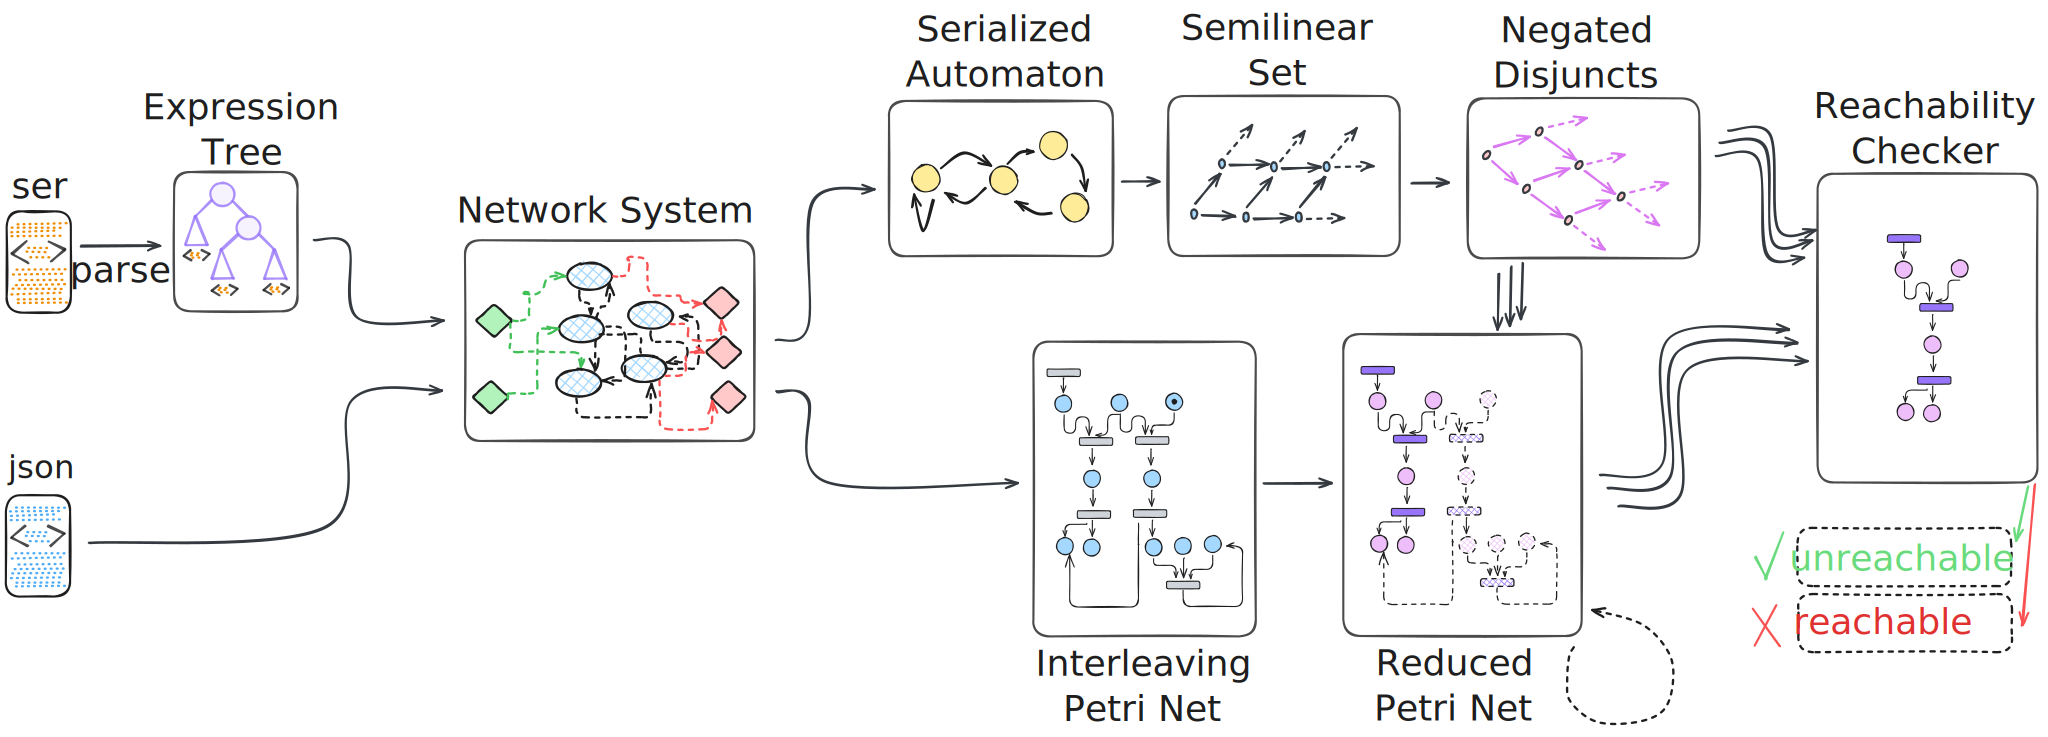
\includegraphics[width=1.0\textwidth]{plots/full_program_flow.pdf}
	\caption{The full decision procedure scheme 
%		If the target set is unreachable --- a serializability proof is produced; otherwise, if it is reachable --- a counterexample trace is generated.
	(simplified version, excluding backward arrows 
%	translating invariants (if serializable) or counterexample traces (if non-serializable) back 
	to the network system level).}
	\label{fig:full_program_flow}
\end{figure}


%\subsection{Optimizations}

%\paragraph{Bidirectional Pruning of the Petri Net}
%Before any heavy symbolic reasoning takes place, we apply bidirectional pruning on the underlying PN.  In the forward pass, we traverse from the initial marking to identify all places and transitions that could ever fire; in the backward pass, we traverse backward from any place that can influence a target constraint, and identify transitions and places that cannot contribute to reaching it.  By iteratively repeating forward passes and backward passes until convergence, we remove every component of the net that cannot both originate and contribute to the reachable target set.  This dramatically shrinks the net in practice, often converting an intractably large model into one small enough for exhaustive analysis.
%%
%We depict this in Fig.~\ref{fig:bidirectional_pruning}, and give a formal proof of correctness in Appendix~\ref{appendix:BidirectionalProof}.

%\paragraph{Redundant‐Constraint Elimination}
%When manipulating Presburger sets or their semilinear representations, it is common for some inequalities or disjuncts to add no new coverage beyond what other constraints already guarantee.  The redundant‐constraint elimination pass inspects each linear inequality and each disjunct in a disjunctive normal form, testing whether it is implied by the rest.  Any constraint or disjunct found redundant is dropped, ensuring that subsequent intersection, union, and projection operations work on the smallest necessary formula.  This streamlines the logic formula and prevents exponential blow‐up of case distinctions during solver invocations.
%
%Every time you build or star a semilinear set, you prune out any “period” vectors that are rendered useless by earlier steps:. nce you’ve accumulated a bunch of LinearSet components, you try to merge any that mathematically subsume one another:

%\paragraph{Generating Fewer Constraints}
%During set‐construction--- especially when introducing new existentially‐quantified variables or combining transition effects, we selectively avoid generating any marking that would strictly dominate an already‐seen solution.  In effect, whenever a candidate disjunct would yield a superset of an existing one, it is skipped entirely.  This ``generate‐less” heuristic stops the proliferation of large, overlapping regions in the semilinear description, trading off completeness of intermediate case‐enumeration for concise final representations.  In benchmarks with large state‐spaces, it can reduce the number of intermediate branches by orders of magnitude.

%in both the Regex and SemilinearSet Kleene-algebra instances. Concretely, instead of always building the full new structure and pruning it later, operations like union (plus) and concatenation (times) do a quick check for trivial cases and drop “zero” or “one” elements on the spo

%\paragraph{Executing Kleene Elimination in a Strategic Order:}
%When converting an NFA to a single regex, we pick the next state to eliminate by heuristically choosing the  state with the fewest incoming and outgoing edges.
%This optimization allows circumventing 
%overblown expressions resulting in naive translations, especially with regard to  Kleene closures (the “\(\mathsf{*}\)” operator).  Instead, we analyze the structure of sub-expressions under the various operators --- estimating their branching factor, and reorder them so that simpler, low‐branching components are expanded first.  This adaptive ordering often leads to early detection of fixed points or dead‐ends, preventing the combinatorial explosion that arises when complex loops are expanded prematurely.  



\subsection{SMPT}
For the underlying Petri net model checker, we use \texttt{SMPT}~\cite{AmDa23}, though other off-the-shelf solvers can be used as well.
%
\texttt{SMPT} incorporates a portfolio of symbolic model checking techniques --- including bounded model checking (BMC)~\cite{BiCiClZh99}, state equation reasoning~\cite{Mu77}, $k$-induction~\cite{BeDaWe18,ShSiSt20}, property directed reachability (PDR)~\cite{Br11,AmDaHu22,ViGu14,BjGa15,BlLa23,CiGrMoTo14,CiGrMoTo16,DuRo17}, and random state space exploration. It acts as a front-end to an \texttt{SMT} solver (\texttt{Z3}~\cite{DeBj08}, although other solvers could also be used, e.g., \texttt{cvc5}~\cite{BaCoDeHaJoKiReTi11,BaBaBrKrLaMaMoMoNiNo22}, \texttt{MathSAT}~\cite{CiGrScSe13}, etc.), while also incorporating domain-specific knowledge from Petri net theory, such as invariants and structural properties. \texttt{SMPT} has also participated in the last five editions of the \textit{Model Checking Contest} (MCC), an international competition for model-checking tools. In its most recent participation, it achieved a bronze medal and a confidence level score of  $\texttt{100\%}$, indicating it never returned an incorrect verdict~\cite{mcc:2025}.

\medskip
\noindent
\texttt{SMPT} distinguishes itself from other tools in two ways that are particularly relevant to our setting and motivate its adoption. First, to the best of our knowledge, it is the only model checker for Petri nets that provides a proof of its verdict, regardless of the underlying verification technique. This means it either produces a witness trace when the property is reachable, or, more interestingly, a certificate of non-reachability~\cite{AmDaHu22} when the property is found to be unreachable.
%
The second distinguishing feature relates to our ongoing work on polyhedral reductions~\cite{AmBeDa21,amat2022polyhedral}, as elaborated further in~\Cref{sec:discussion}.


\subsection{Benchmarks} 
\label{subsec:benchmarks}
To the best of our knowledge, ours is the first and only tool capable of (i) checking serializability on programs running \textit{unbounded} threads; and (ii) \textit{proving that serializability holds}.
%
Thus, we have found a lack of standard serializability benchmarks for evaluating our tool. Towards this end, we bridged this gap in the literature by assembling a suite of dozens of benchmarks (which we also uploaded online~\cite{ArtifactRepository}).
% additional part (from rebuttal to R4) - END
%Typically, automatically generated $\toolname$ programs do not represent real-world applications or recognizable concurrency patterns. Thus, 
We believe that this is the first benchmark suite for serializability, and includes instances of \toolname{} programs that are motivated by practical, real-world analogues.
% additional part (from rebuttal to R4) - END
Specifically, our suite includes both \texttt{SER} and \texttt{JSON} formatted programs, with both serializable and non-serializable instances.
%
Furthermore, our benchmarks (see Table~\ref{tab:benchmarks-all}) cover a broad range of features, including loops, branching, arithmetic, locks, non-determinism, and more.
%
While the benchmarks are not the paper’s primary focus, we believe they stand on their own, given their strong relevance to a range of real-world systems and applications of interest.
%
In particular, we highlight our benchmark suite encoding \textit{network \& system protocols}, which includes models of real-world BGP routing programs, stateful firewalls, asynchronous network monitors, and additional
%highlighting the serializability challenges inherent in real-world distributed programs.
%
%Here, we were motivated by 
examples motivated by real-world concurrency problems. 
%
For example, our \textit{routing-cycle benchmark} in SDN is motivated by a recent networking paper~\cite{NaGhSa24}. Another interesting example is illustrated by our \textit{snapshot isolation benchmark} --- motivated by a reported duplicate-key bug~\cite{cockroach-issue-14099} in the \texttt{CockroachDB} system~\cite{cockroachdb-si-docs}.
%
In both cases and others, the unwanted behavior was expressed by serializability violations that our toolchain successfully and automatically identified.
%
%Our benchmarks include both serializable and non-serializable instances, and their features and categorization appears in Table~\ref{tab:benchmarks-all}. 



%As there are no standard benchmarks for evaluating serializability, we wrote dozens of programs in our abstract NS language. These benchmarks span a wide range of complexity --- covering branching, looping constructs, arithmetic, non-deterministic choice, and multi-request workflows that manipulate both shared (global) variables and per-request (local) state. 
%
%We include both serializable and non-serializable instances and summarize the benchmarks' features and categorizations in Table~\ref{tab:benchmarks-all}. 
%
%In particular, our most sophisticated examples are drawn from realistic networking and system-protocol scenarios, including stateful firewalls, BGP routing, network monitoring, and more --- highlighting the serializability challenges inherent in real-world distributed programs.
%
%As there are no official benchmarks for evaluating serializability, we hand-coded dozes of programs in our abstract network-system language.
%%
%The benchmarks vary in the complexity, and have multiple features: branching, loops, arithmetic, non-determinism, and multiple requests and responses, operating on both shared (global) variables and per-request (local) variables.
%%
%The benchmarks include both serializable and non-serializable instances, as we summarize in Table.~\ref{tab:benchmarks-all}, based on a category and feature-wise breakdown.
%%
%Especially, we wish to note the final category of complex examples as motivated by real-world systems and networking programs.
%%
%These include a stateful firewall, BGP routing, network monitoring and additional examples.
%
%\begin{itemize}
%		
%	\item \todo{update benchmark overview and category names}
%	\item \textbf{Core expressions \& multi request workflows}: Benchmarks testing arithmetic, boolean, and simple control expression.
%	\item \textbf{Fred (mixed arithmetic)}: Mixed control and arithmetic transformations (Fred series).
%	\item \textbf{Stop (circular-increment) series}: Circular increment loops and variants.
%	\item \textbf{Concurrency \& locking loops}: Concurrent looping patterns with locking and tricky interactions.
%	\item \textbf{Non-deterministic choice \& randomness}: Random choice and non-deterministic branching benchmarks.
%	\item \textbf{Networking \& system protocols}: Networking protocols and system-level monitoring.
%	\item \textbf{JSON state-machine examples}: Example JSON-encoded state machine workflows.
%\end{itemize}
%
%
%
%The benchmarks differ in their complexity and in the various features pertaining to them --- branching, loops, randomness, multiple requests, etc. 
%

	

%\newpage